\documentclass{standalone}
%\documentclass[a4paper,aps,prl,onecolumn]{revtex4}

\usepackage{graphicx} %[dvips]
\usepackage[usenames,dvipsnames]{xcolor}

\usepackage{tikz}
\usepackage{amsmath}
\usepackage{amssymb}
%\usepackage{natbib}
%\usepackage{color}
%\usepackage{float}
%\usepackage{epstopdf}
\usepackage[normalem]{ulem}
\usepackage{pgfplots,pgfplotstable}
\usepackage{hyperref}
\usepackage{soul}
\usepackage{comment}
\usepgfplotslibrary{fillbetween}

\usetikzlibrary[shadings]
\usetikzlibrary{shapes}
\usetikzlibrary{snakes}
\usetikzlibrary {arrows.meta}

%% A text box with a white background and rounded edges
\newcommand*{\wbox}[1]{%
	\tikz[baseline=(X.base)] \node[rectangle, fill=white, rounded corners, inner sep=0.6mm] (X) {#1};%
}

\newcommand{\vett}[1]{\mathbf{#1}}
\newcommand {\Curl} {\mbox{\rm curl\,}}
\newcommand {\Skw} {\mbox{\rm skw\,}}
\newcommand {\Sym} {\mbox{\rm $\mathbb{S}$ym\,}}
\newcommand {\PSym} {\mbox{\rm P$\mathbb{S}$ym\,}}
\newcommand {\Lin} {\mbox{\rm $\mathbb{L}$in\,}}
\newcommand {\sym} {\mbox{\rm sym\,}}
\newcommand {\Div} {\mbox{\rm div\,}}
\newcommand {\tr} {\mbox{\rm tr\,}}
\newcommand {\sph} {\mbox{\rm sph\,}}
\newcommand {\sgn} {\mbox{\rm sgn\,}}
\newcommand{\minus}{\scalebox{0.6}[1.0]{$-$}}
\newenvironment{sistema}%
{\left\lbrace\begin{array}{@{}l@{}}}%
{\end{array}\right.}

\definecolor{IBM1}{HTML}{648fff}
\definecolor{IBM2}{HTML}{785ef0}
\definecolor{IBM3}{HTML}{dc267f}
\definecolor{IBM4}{HTML}{fe6100}
\definecolor{IBM5}{HTML}{ffb000}
\definecolor{IBM6}{RGB}{051,117,056}

\definecolor{Okabe1}{RGB}{000,158,115}
\definecolor{Okabe2}{RGB}{000,114,178}
\definecolor{Okabe3}{RGB}{086,180,233}
\definecolor{Okabe4}{RGB}{230,159,000}
\definecolor{Okabe5}{RGB}{213,094,000}
\definecolor{Okabe6}{RGB}{204,121,167}

\definecolor{b1}{HTML}{d73027}
\definecolor{b2}{HTML}{fc8d59}
\definecolor{b3}{HTML}{fee090}
\definecolor{b4}{HTML}{e0f3f8}
\definecolor{b5}{HTML}{91bfdb}
\definecolor{b6}{HTML}{4575b4}


\begin{document}



\pgfplotsset{compat=newest}

\begin{tikzpicture}
\label{Lp}
\begin{axis}[
	%axis background/.style={fill=gray!10},
	enlargelimits=false,
	%ylabel near ticks,
	title={$c.$},
	title style={yshift=-2ex, xshift=-35ex},
	tick pos=left, %
	tick align=outside, %
	axis line style={opacity=0}, %
	after end axis/.code={
		\draw ({rel axis cs:0,0}
		-|{axis cs:0.59,0}) % xmin (line starts here)
		-- ({rel axis cs:0,0}
		-|{axis cs:0.62,0}); % xmax (line stops here)
		\draw ({rel axis cs:0,0}
		|-{axis cs:0,0}) % ymin (line starts here)
		-- ({rel axis cs:0,0}
		|-{axis cs:0,1}); % ymax (line stops here)
	},
	grid=none,
	x label style={at={(axis description cs:0.5,-0.1375)},anchor=north},
	%y label style={at={(axis description cs:-.075,.45)},rotate=0,anchor=south}, %shiftin relative to axis
	xlabel style={yshift=0.3cm},
	xlabel={$\phi_0$},
	ylabel={$P$ (force chain formed)},
	xmin=0.588,
	xmax=0.62,
	ymin=-0.05,
	ymax=1.0,
	legend style={at={(0.025,1)},anchor=north west},
	%legend image post style={scale=0.5},
	ytick={0, 0.25, 0.5, 0.75, 1},
	yticklabels = {0, 0.25, 0.5, 0.75, 1},
	y tick label style={
		/pgf/number format/.cd,
		fixed,
		fixed zerofill,
		precision=0,
		/tikz/.cd
	},
	xtick={0.59, 0.6, 0.606491, 0.61, 0.62},
	xticklabels = {0.59, 0.6, $\phi_f$, 0.61, 0.62},
	x tick label style={
		/pgf/number format/.cd,
		fixed,
		fixed zerofill,
		precision=0,
		/tikz/.cd
	},
	%yticklabel={\ifdim\tick pt=0pt 0 \else\pgfmathprintnumber{\tick}\fi},
	%xticklabel={\ifdim\tick pt=0pt 0 \else\pgfmathprintnumber{\tick}\fi}
	]

]
	%\addplot[color = b1, ultra thick]  table[x index = 1, y index = 2, col sep=comma]{chains_results.csv};
	
	\addplot[name path=A, domain=0.55:0.7, samples=5, color = Okabe1!50, thick]  table[skip first n = 1, x index = 1, y index = 9, col sep=comma]{chains_results_10-26-26.csv};
	\addplot[name path=B, domain=0.55:0.7, samples=5, color = Okabe1!50, thick]  table[skip first n = 1, x index = 1, y index = 10, col sep=comma]{chains_results_10-26-26.csv};
	\addplot[color=Okabe1!50] fill between [of=A and B];
	\addplot[color = Okabe1, thick]  table[skip first n = 1, x index = 1, y index = 7, col sep=comma]{chains_results_10-26-26.csv};
	%\addplot[color = b3, ultra thick]  table[x index = 1, y index = 4, col sep=comma]{chains_results.csv};
	
	\addplot[domain=-0.05:1, samples=2, dashed, black] ({0.606491}, {x});
	
	
	
	%\addplot[color = Black!50, ultra thick]  table[x index = 37, y index = 38, col sep=comma]{results_file.csv};
	%\addplot[color = gradient7, ultra thick]  table[x index = 6, y index = 13, col sep=comma]{results_file.csv};

	% Draw an arrow (xi, yi) to (xf, yf)
	%\draw[->] (2, 15.5) -- (9, 15.5);

	% Add text. \wbox puts a white box behind it so it can go over a curve, if you want
	%\node [anchor=west] at (axis cs: 14.5, 5.6) {\color{Okabe1}{\wbox{\footnotesize{--- 0 kPa}}}}; %16.6, 16.77, 16.51, 16.58, 16.63, 16.38
	%\node [anchor=west] at (axis cs: 14.5, 8.65) {\color{Okabe2}{\wbox{\footnotesize{--- 5 kPa}}}};
	%\node [anchor=west] at (axis cs: 14.5, 10.45) {\color{Okabe3}{\wbox{\footnotesize{--- 10 kPa}}}};		
	%\node [anchor=west] at (axis cs: 14.5, 12){\color{Okabe4}{\wbox{\footnotesize{--- 15 kPa}}}};		
	%\node [anchor=west] at (axis cs: 14.4, 12.75){\color{Okabe5}{\wbox{\footnotesize{--- 20 kPa}}}};		
	%\node [anchor=west] at (axis cs: 14.3, 14.4){\color{Okabe6}{\wbox{\footnotesize{--- 25 kPa}}}};	
	
	
	%\node at (axis cs: 16.01, 20.29) {\color{gradient7}{\wbox{\footnotesize{--- 30 kPa}}}};
	
	%\addplot[domain=0.5:3.5, thick, black] {0.90*x};
	%\addplot[domain=0.5:3.5, thick, black] {0.35*x};
	
	% Plot the right triangle
	%\addplot[mark=none, thick,black] coordinates {(-.05,-.05) (-.05,2.6) (3.188,2.6) (-.05,-.05)};	
	%\addplot[mark=none, thick,black] coordinates {(-.08,-.05) (3.188,-.05) (3.188,1.275) (-.07,-.05)};
	
	% Annotate the triangle sides
	%\node at (axis cs:1.45,3.1) [black]{$k$};
	%\node at (axis cs:3.75,0.625) [black]{$k_o$};
	
	% Plot F_c
	%\addplot[domain=0:10.38, dashed, black] {11.53};
	
	% Plot del_c
	%\addplot[domain=0:11.53, samples=2, dashed, black] ({10.38}, {x});
	
	\node[anchor=west] at (0.59, 0.666) {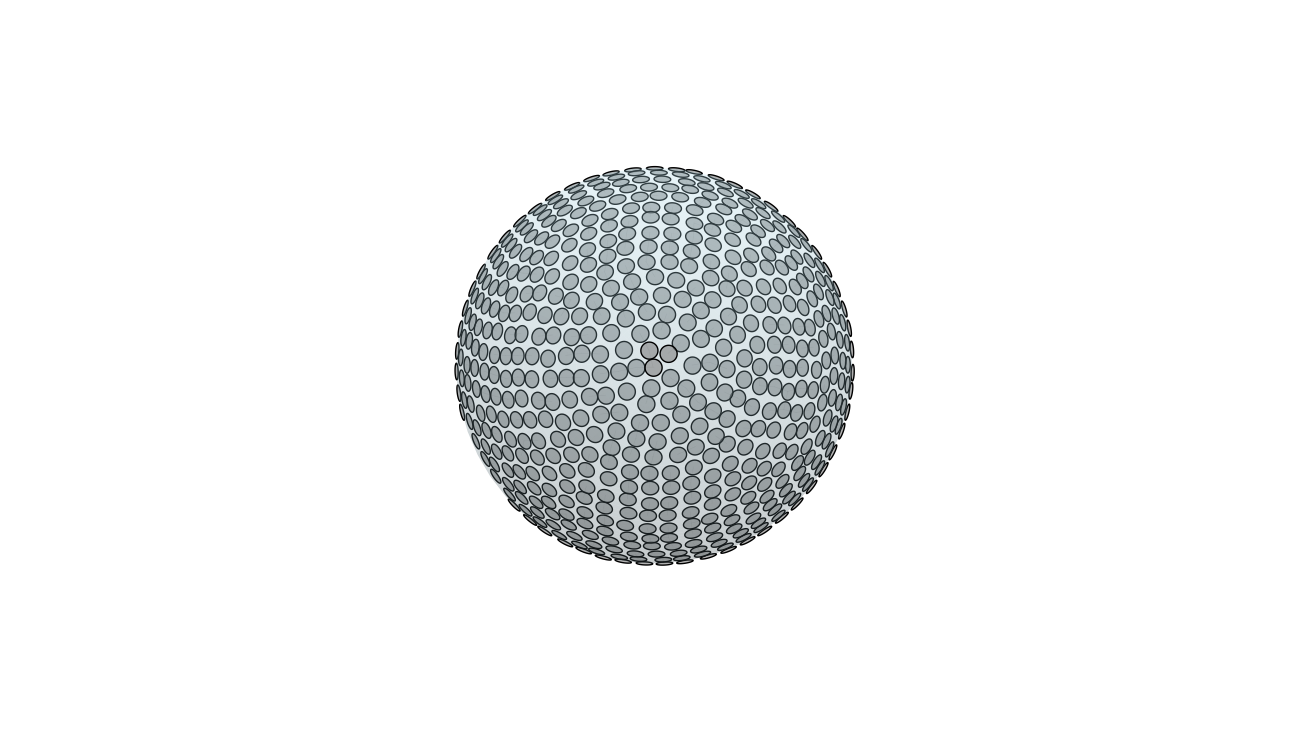
\includegraphics[width=2.5cm,trim=300 90 300 90,clip]{0.59_topDown}};
	%\addplot[mark=none, thick,black] coordinates {(0.565,0.12) (0.585,0)};	
	%\draw[-Stealth] (0.56,0.55) -- (0.584,0.005);
	

	
	\node[anchor=east] at (0.62, 0.333) {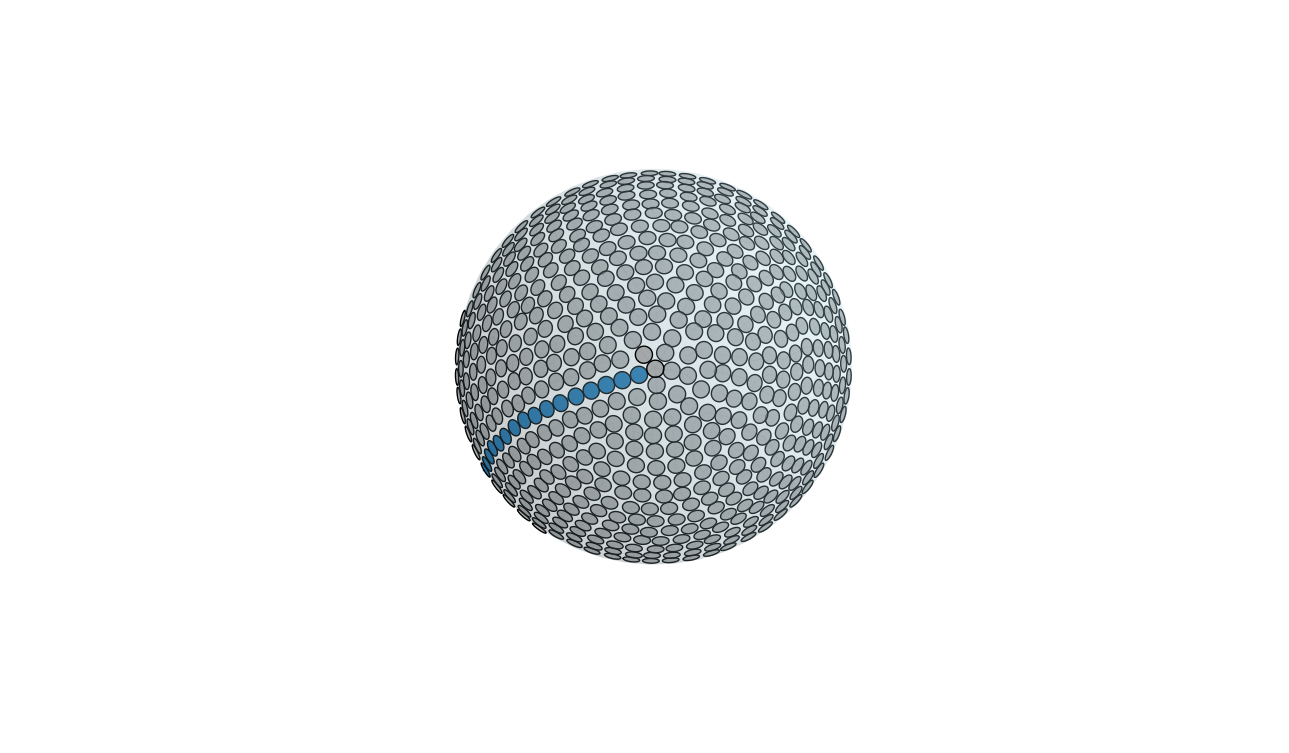
\includegraphics[width=2.5cm,trim=300 90 300 90,clip]{0.62_topDown}};
	%\draw[-Stealth] (0.72, 0.659) -- (0.663,0.995);
	
	%\node[anchor=center] at (2.5, 5) {\includegraphics[width=2cm]{unindentedShell}};
	%\node[anchor=center] at (4, 9) {\includegraphics[width=3cm]{flatCapShell}};
	%\node[anchor=center] at (15, 2) {\includegraphics[width=3cm]{invertedShell}};
	
	%\addlegendentry[scale=0.75]{1.05}
		%\addlegendentry[scale=0.75]{1.136}
	%\addlegendentry[scale=0.75]{1.15}
	
	%\addlegendentry[scale=0.75]{10 kPa}
	%\addlegendentry[scale=0.75]{5 kPa}
	%\addlegendentry[scale=0.75]{0 kPa}
	%\addlegendentry[scale=0.75]{empty}
	

\end{axis}	

\end{tikzpicture}

\end{document}